\documentclass[12pt]{article}

\usepackage[utf8]{inputenc}
\usepackage[T1]{fontenc}
\usepackage[spanish]{babel}
\usepackage[margin=2.5cm]{geometry}
\usepackage{booktabs}      
\usepackage{listings}      
\usepackage{xcolor}
\usepackage{graphicx}      
\usepackage{xurl}
\usepackage[hidelinks]{hyperref}
\usepackage{bookmark}

% ============================================================
% Configuración de bloques de código (para el Apéndice)
% ============================================================
\lstset{
    language=Python,
    basicstyle=\ttfamily\small,
    keywordstyle=\color{blue},
    commentstyle=\color{gray},
    stringstyle=\color{teal},
    numbers=left,
    numberstyle=\tiny,
    frame=single,
    breaklines=true,
    showstringspaces=false,
    % ======= OPCIONES PARA UTF-8 =======
    inputencoding=utf8,
    extendedchars=true,
    literate=
      {á}{{\'a}}1 {é}{{\'e}}1 {í}{{\'i}}1 {ó}{{\'o}}1 {ú}{{\'u}}1
      {Á}{{\'A}}1 {É}{{\'E}}1 {Í}{{\'I}}1 {Ó}{{\'O}}1 {Ú}{{\'U}}1
      {ñ}{{\~n}}1 {Ñ}{{\~N}}1
}

% ============================================================
% Portada
% ============================================================
\title{[Título tentativo del proyecto]}
\author{Angie Montero \and Michael Baquero}
\date{Analítica Descriptiva II \\ \large Unicafam \\ Agosto 2026}

\begin{document}

\maketitle

% ============================================================
% SALTO DE PÁGINA PARA SEPARAR LA PORTADA
% ============================================================
\newpage

% ============================================================
% 1. Introducción
% ============================================================
\section{Introducción}

% ============================================================
% SALTO DE PÁGINA PARA SEPARAR LA INTRODUCCIÓN DEL DESARROLLO
% ============================================================
\newpage

% ============================================================
% 2. Descripción del dataset (Con desarrollo narrativo completo)
% ============================================================
\section{Descripción del dataset}

Los datos utilizados en este estudio provienen de la base de
\textbf{Estadísticas de Comercio Exterior -- Exportaciones}, publicada
por la Dirección de Impuestos y Aduanas Nacionales (DIAN), validada y
certificada por el Departamento Administrativo Nacional de Estadística
(DANE). Corresponde al mes de junio de 2026 y fue descargada el 12 de
agosto de 2026 desde
\href{https://www.dian.gov.co/dian/cifras/Paginas/Bases-Estadisticas-de-Comercio-Exterior-Importaciones-y-Exportaciones.aspx}{la página oficial de estadísticas de comercio exterior de la DIAN}.

El archivo original contiene un total de 103.179 registros y 72 variables. 
Dentro de este conjunto de datos, se identificaron 44 columnas de tipo numérico y 28 columnas de tipo categórico o texto, tal como se resume en la Tabla~\ref{tab:resumen_original}.

\begin{figure}[h!]
    \centering
    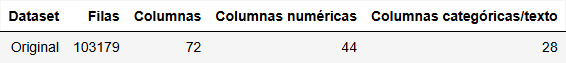
\includegraphics[width=0.7\textwidth]{anexos/tabla_resumen_original.png}
    \caption{Resumen del dataset original de exportaciones (junio 2026).}
    \label{tab:resumen_original}
\end{figure}

\subsection*{Exploración de variables categóricas}
Para determinar qué variables categóricas eran adecuadas para las
pruebas de hipótesis del proyecto, se realizó una exploración inicial
sobre las variables candidatas: \texttt{MODO\_TRANSPORTE},
\texttt{MODALIDAD\_EXPORTACION}, \texttt{PAIS\_DESTINO\_FINAL},
\texttt{REGION\_DE\_ORIGEN} y \texttt{TIPO\_DE\_EMBARQUE}. El objetivo
fue evaluar el número de categorías únicas presentes en cada una, ya que
un número excesivo de categorías dificulta el análisis estadístico
(Tabla~\ref{tab:categoricas}).

\begin{figure}[h!]
    \centering
    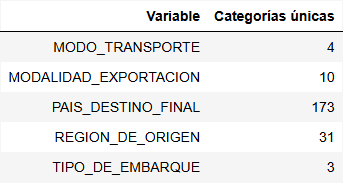
\includegraphics[width=0.5\textwidth]{anexos/tabla_categoricas.png}
    \caption{Número de categorías únicas por variable categórica candidata.}
    \label{tab:categoricas}
\end{figure}

Con base en este análisis, se identificó que la variable
\texttt{PAIS\_DESTINO\_FINAL} presenta un total de 173 categorías
únicas. Esta alta cardinalidad la hace estadísticamente inviable para
pruebas de hipótesis del tipo chi-cuadrado, ya que generaría una matriz
de contingencia demasiado dispersa y sin poder explicativo. Por lo tanto,
se decidió excluirla del análisis.

\subsection*{Selección de variables finales}
Tras la exclusión de \texttt{PAIS\_DESTINO\_FINAL}, se seleccionaron
11 variables relevantes que orientan el desarrollo de la pregunta de
investigación y el modelo de regresión final. Esta selección incluye
tanto variables cuantitativas (como valores monetarios y pesos) como
variables categóricas de baja cardinalidad. La descripción técnica de
cada variable seleccionada se presenta en la Tabla~\ref{tab:variables_seleccionadas}.

\begin{figure}[h!]
    \centering
    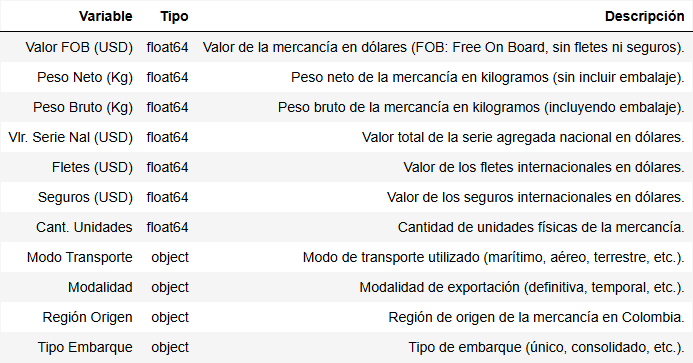
\includegraphics[width=0.9\textwidth]{anexos/tabla_variables_seleccionadas.png}
    \caption{Variables seleccionadas del dataset de exportaciones.}
    \label{tab:variables_seleccionadas}
\end{figure}

\subsection*{Muestreo y dimensiones finales}
Dado el volumen del dataset filtrado y con el fin de optimizar los
recursos computacionales, se optó por trabajar con una muestra aleatoria
simple de 1.500 registros. Se fijó una semilla aleatoria
(\texttt{random\_state=42}) para garantizar la reproducibilidad de los
resultados. Esta reducción evita sobrecargar el modelo de regresión
lineal y reduce significativamente los tiempos de ejecución. La
comparación de las dimensiones del dataset filtrado frente a la muestra
de trabajo se observa en la Tabla~\ref{tab:dimensiones_muestra}.

\begin{figure}[h!]
    \centering
    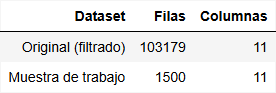
\includegraphics[width=0.6\textwidth]{anexos/tabla_dimensiones_muestra.png}
    \caption{Comparación de dimensiones: dataset filtrado vs. muestra de trabajo (n=1500).}
    \label{tab:dimensiones_muestra}
\end{figure}

A modo de ejemplo tangible, la Tabla~\ref{tab:muestra_head} presenta
las primeras cinco filas de la muestra de trabajo. Se puede observar
cómo se estructuran los datos de las variables cuantitativas y
categóricas seleccionadas para el estudio.

\begin{figure}[h!]
    \centering
    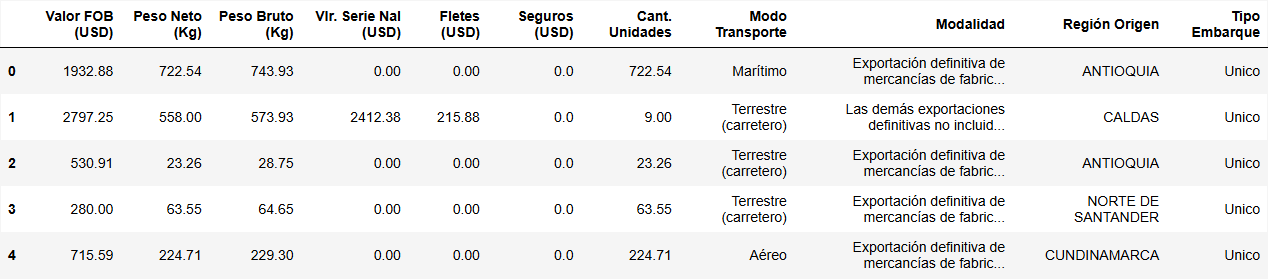
\includegraphics[width=0.85\textwidth]{anexos/tabla_muestra_head.png}
    \caption{Primeras 5 filas de la muestra de trabajo (n=1500).}
    \label{tab:muestra_head}
\end{figure}

% ============================================================
% SALTO DE PÁGINA PARA SEPARAR LO DESARROLLADO DE LO PENDIENTE
% ============================================================
\newpage

% ============================================================
% 3. Análisis exploratorio (EDA)
% ============================================================
\section{Análisis exploratorio}

% TODO (Angie): tabla de estadística descriptiva (media, mediana,
% desviación estándar, mínimo, máximo, asimetría) + su interpretación.
\subsection{Estadística descriptiva}

% TODO (Angie): mínimo 2 visualizaciones con interpretación escrita.
\subsection{Visualizaciones}

% TODO (Michael): verificación de normalidad (Shapiro-Wilk + gráfico Q-Q)
% para al menos una variable cuantitativa.
\subsection{Verificación de normalidad}

% ============================================================
% SALTO DE PÁGINA ANTES DE LAS REFERENCIAS Y EL APÉNDICE
% ============================================================
\newpage

% ============================================================
% Referencias
% ============================================================
% TODO (Michael): mínimo 4 referencias APA 7ª ed. (2 académicas + 2 de
% fuentes de datos).
\section*{Referencias}

% ============================================================
% SALTO DE PÁGINA PARA EL APÉNDICE
% ============================================================
\newpage

% ============================================================
% Apéndices
% ============================================================
\appendix
\section{Apéndice: Código fuente}

% TODO (Michael): pegar aquí el contenido de eda_exportaciones.py
% usando \lstinputlisting o \begin{lstlisting}...\end{lstlisting}
\lstinputlisting[language=Python]{../eda_exportaciones.py}

\end{document}